
头文件<version>允许请求编译器提供C++11或更高版本的支持。可以查询核心语言或库的属性、特性。<version>定义了大约200个宏,这些宏在实现特性时扩展为一个数字。这个数字代表该特性添加到C++标准中的年份和月份。这些是static\_assert、Lambda和概念的数字。

\hspace*{\fill} \\ %插入空行
\noindent
\textbf{用于表示static\_assert、Lambda和概念的宏}
\begin{lstlisting}[style=styleCXX]
__cpp_static_assert 200410L
__cpp_lambdas 200907L
__cpp_concepts 201907L
\end{lstlisting}

\begin{tcolorbox}[breakable,enhanced jigsaw,colback=blue!5!white,colframe=blue!75!black,title={支持的功能}]
	
当尝试全新的C++特性时,我会检查哪个编译器实现了我感兴趣的特性。这是我访问\href{https://en.cppreference.com/w/cpp/compiler_support}{cppreference.com/compiler\_support}的时候,搜索我想尝试的功能,并希望三大编译器(GCC, Clang, MSVC)中至少有一个实现了新功能。

\hspace*{\fill} \\ %插入空行
只得到部分答案并不令人满意。最后,当一个全新功能的编译失败时,我也不知道该去找谁。
\end{tcolorbox}

\begin{center}
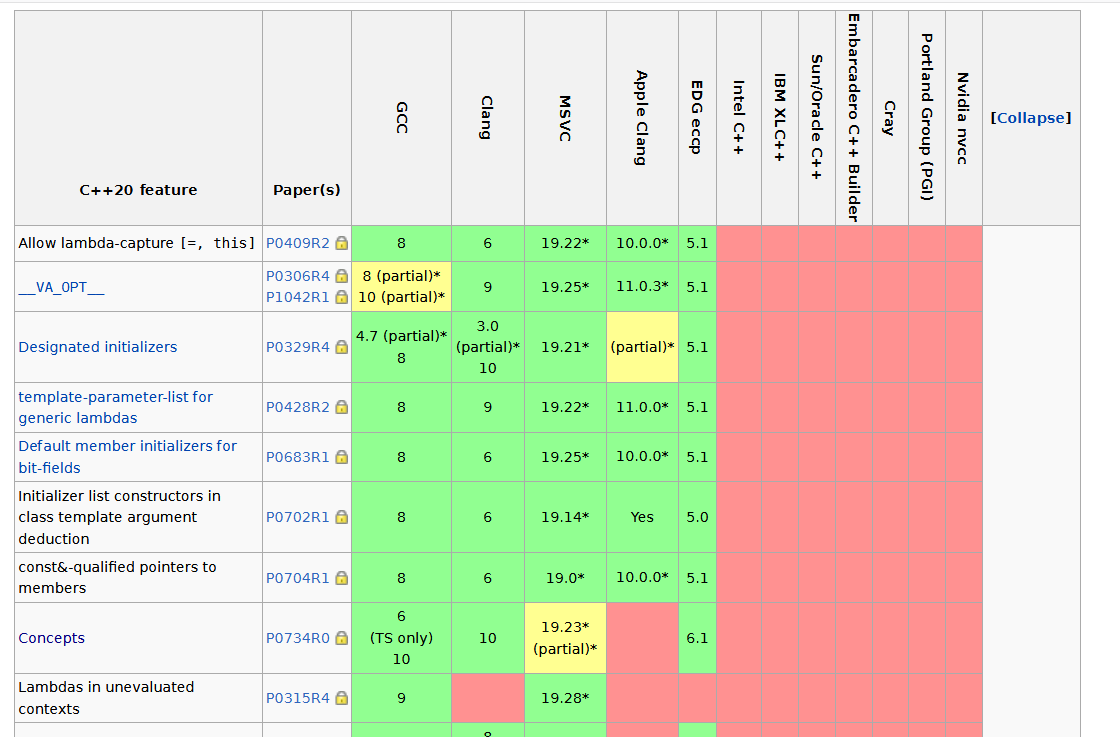
\includegraphics[width=1.0\textwidth]{content/5/chapter9/images/1.png}\\
支持C++20核心语言的特性
\end{center}

cppreference.com的\href{https://en.cppreference.com/w/cpp/feature_test}{功能测试}页面,在一个很长的源文件中使用了所有宏。

\begin{lstlisting}[style=styleCXX]
// featureTest.cpp
// from cppreference.com

#if __cplusplus < 201100
# error "C++11 or better is required"
#endif

#include <algorithm>
#include <cstring>
#include <iomanip>
#include <iostream>
#include <string>

#ifdef __has_include
# if __has_include(<version>)
# include <version>
# endif
#endif

#define COMPILER_FEATURE_VALUE(value) #value
#define COMPILER_FEATURE_ENTRY(name) { #name, COMPILER_FEATURE_VALUE(name) },

#ifdef __has_cpp_attribute
# define COMPILER_ATTRIBUTE_VALUE_AS_STRING(s) #s
# define COMPILER_ATTRIBUTE_AS_NUMBER(x) COMPILER_ATTRIBUTE_VALUE_AS_STRING(x)
# define COMPILER_ATTRIBUTE_ENTRY(attr) \
	{ #attr, COMPILER_ATTRIBUTE_AS_NUMBER(__has_cpp_attribute(attr)) },
#else
# define COMPILER_ATTRIBUTE_ENTRY(attr) { #attr, "_" },
#endif

// Change these options to print out only necessary info.
static struct PrintOptions {
	constexpr static bool titles = 1;
	constexpr static bool attributes = 1;
	constexpr static bool general_features = 1;
	constexpr static bool core_features = 1;
	constexpr static bool lib_features = 1;
	constexpr static bool supported_features = 1;
	constexpr static bool unsupported_features = 1;
	constexpr static bool sorted_by_value = 0;
	constexpr static bool cxx11 = 1;
	constexpr static bool cxx14 = 1;
	constexpr static bool cxx17 = 1;
	constexpr static bool cxx20 = 1;
	constexpr static bool cxx23 = 0;
} print;

struct CompilerFeature {
	CompilerFeature(const char* name = nullptr, const char* value = nullptr)
		: name(name), value(value) {}
	const char* name; const char* value;
};

static CompilerFeature cxx[] = {
COMPILER_FEATURE_ENTRY(__cplusplus)
COMPILER_FEATURE_ENTRY(__cpp_exceptions)
COMPILER_FEATURE_ENTRY(__cpp_rtti)
#if 0
COMPILER_FEATURE_ENTRY(__GNUC__)
COMPILER_FEATURE_ENTRY(__GNUC_MINOR__)
COMPILER_FEATURE_ENTRY(__GNUC_PATCHLEVEL__)
COMPILER_FEATURE_ENTRY(__GNUG__)
COMPILER_FEATURE_ENTRY(__clang__)
COMPILER_FEATURE_ENTRY(__clang_major__)
COMPILER_FEATURE_ENTRY(__clang_minor__)
COMPILER_FEATURE_ENTRY(__clang_patchlevel__)
#endif
};
static CompilerFeature cxx11[] = {
COMPILER_FEATURE_ENTRY(__cpp_alias_templates)
COMPILER_FEATURE_ENTRY(__cpp_attributes)
COMPILER_FEATURE_ENTRY(__cpp_constexpr)
COMPILER_FEATURE_ENTRY(__cpp_decltype)
COMPILER_FEATURE_ENTRY(__cpp_delegating_constructors)
COMPILER_FEATURE_ENTRY(__cpp_inheriting_constructors)
COMPILER_FEATURE_ENTRY(__cpp_initializer_lists)
COMPILER_FEATURE_ENTRY(__cpp_lambdas)
COMPILER_FEATURE_ENTRY(__cpp_nsdmi)
COMPILER_FEATURE_ENTRY(__cpp_range_based_for)
COMPILER_FEATURE_ENTRY(__cpp_raw_strings)
COMPILER_FEATURE_ENTRY(__cpp_ref_qualifiers)
COMPILER_FEATURE_ENTRY(__cpp_rvalue_references)
COMPILER_FEATURE_ENTRY(__cpp_static_assert)
COMPILER_FEATURE_ENTRY(__cpp_threadsafe_static_init)
COMPILER_FEATURE_ENTRY(__cpp_unicode_characters)
COMPILER_FEATURE_ENTRY(__cpp_unicode_literals)
COMPILER_FEATURE_ENTRY(__cpp_user_defined_literals)
COMPILER_FEATURE_ENTRY(__cpp_variadic_templates)
};
static CompilerFeature cxx14[] = {
COMPILER_FEATURE_ENTRY(__cpp_aggregate_nsdmi)
COMPILER_FEATURE_ENTRY(__cpp_binary_literals)
COMPILER_FEATURE_ENTRY(__cpp_constexpr)
COMPILER_FEATURE_ENTRY(__cpp_decltype_auto)
COMPILER_FEATURE_ENTRY(__cpp_generic_lambdas)
COMPILER_FEATURE_ENTRY(__cpp_init_captures)
COMPILER_FEATURE_ENTRY(__cpp_return_type_deduction)
COMPILER_FEATURE_ENTRY(__cpp_sized_deallocation)
COMPILER_FEATURE_ENTRY(__cpp_variable_templates)
};
static CompilerFeature cxx14lib[] = {
COMPILER_FEATURE_ENTRY(__cpp_lib_chrono_udls)
COMPILER_FEATURE_ENTRY(__cpp_lib_complex_udls)
COMPILER_FEATURE_ENTRY(__cpp_lib_exchange_function)
COMPILER_FEATURE_ENTRY(__cpp_lib_generic_associative_lookup)
COMPILER_FEATURE_ENTRY(__cpp_lib_integer_sequence)
COMPILER_FEATURE_ENTRY(__cpp_lib_integral_constant_callable)
COMPILER_FEATURE_ENTRY(__cpp_lib_is_final)
COMPILER_FEATURE_ENTRY(__cpp_lib_is_null_pointer)
COMPILER_FEATURE_ENTRY(__cpp_lib_make_reverse_iterator)
COMPILER_FEATURE_ENTRY(__cpp_lib_make_unique)
COMPILER_FEATURE_ENTRY(__cpp_lib_null_iterators)
COMPILER_FEATURE_ENTRY(__cpp_lib_quoted_string_io)
COMPILER_FEATURE_ENTRY(__cpp_lib_result_of_sfinae)
COMPILER_FEATURE_ENTRY(__cpp_lib_robust_nonmodifying_seq_ops)
COMPILER_FEATURE_ENTRY(__cpp_lib_shared_timed_mutex)
COMPILER_FEATURE_ENTRY(__cpp_lib_string_udls)
COMPILER_FEATURE_ENTRY(__cpp_lib_transformation_trait_aliases)
COMPILER_FEATURE_ENTRY(__cpp_lib_transparent_operators)
COMPILER_FEATURE_ENTRY(__cpp_lib_tuple_element_t)
COMPILER_FEATURE_ENTRY(__cpp_lib_tuples_by_type)
};

static CompilerFeature cxx17[] = {
COMPILER_FEATURE_ENTRY(__cpp_aggregate_bases)
COMPILER_FEATURE_ENTRY(__cpp_aligned_new)
COMPILER_FEATURE_ENTRY(__cpp_capture_star_this)
COMPILER_FEATURE_ENTRY(__cpp_constexpr)
COMPILER_FEATURE_ENTRY(__cpp_deduction_guides)
COMPILER_FEATURE_ENTRY(__cpp_enumerator_attributes)
COMPILER_FEATURE_ENTRY(__cpp_fold_expressions)
COMPILER_FEATURE_ENTRY(__cpp_guaranteed_copy_elision)
COMPILER_FEATURE_ENTRY(__cpp_hex_float)
COMPILER_FEATURE_ENTRY(__cpp_if_constexpr)
COMPILER_FEATURE_ENTRY(__cpp_inheriting_constructors)
COMPILER_FEATURE_ENTRY(__cpp_inline_variables)
COMPILER_FEATURE_ENTRY(__cpp_namespace_attributes)
COMPILER_FEATURE_ENTRY(__cpp_noexcept_function_type)
COMPILER_FEATURE_ENTRY(__cpp_nontype_template_args)
COMPILER_FEATURE_ENTRY(__cpp_nontype_template_parameter_auto)
COMPILER_FEATURE_ENTRY(__cpp_range_based_for)
COMPILER_FEATURE_ENTRY(__cpp_static_assert)
COMPILER_FEATURE_ENTRY(__cpp_structured_bindings)
COMPILER_FEATURE_ENTRY(__cpp_template_template_args)
COMPILER_FEATURE_ENTRY(__cpp_variadic_using)
};
static CompilerFeature cxx17lib[] = {
COMPILER_FEATURE_ENTRY(__cpp_lib_addressof_constexpr)
COMPILER_FEATURE_ENTRY(__cpp_lib_allocator_traits_is_always_equal)
COMPILER_FEATURE_ENTRY(__cpp_lib_any)
COMPILER_FEATURE_ENTRY(__cpp_lib_apply)
COMPILER_FEATURE_ENTRY(__cpp_lib_array_constexpr)
COMPILER_FEATURE_ENTRY(__cpp_lib_as_const)
COMPILER_FEATURE_ENTRY(__cpp_lib_atomic_is_always_lock_free)
COMPILER_FEATURE_ENTRY(__cpp_lib_bool_constant)
COMPILER_FEATURE_ENTRY(__cpp_lib_boyer_moore_searcher)
COMPILER_FEATURE_ENTRY(__cpp_lib_byte)
COMPILER_FEATURE_ENTRY(__cpp_lib_chrono)
COMPILER_FEATURE_ENTRY(__cpp_lib_clamp)
COMPILER_FEATURE_ENTRY(__cpp_lib_enable_shared_from_this)
COMPILER_FEATURE_ENTRY(__cpp_lib_execution)
COMPILER_FEATURE_ENTRY(__cpp_lib_filesystem)
COMPILER_FEATURE_ENTRY(__cpp_lib_gcd_lcm)
COMPILER_FEATURE_ENTRY(__cpp_lib_hardware_interference_size)
COMPILER_FEATURE_ENTRY(__cpp_lib_has_unique_object_representations)
COMPILER_FEATURE_ENTRY(__cpp_lib_hypot)
COMPILER_FEATURE_ENTRY(__cpp_lib_incomplete_container_elements)
COMPILER_FEATURE_ENTRY(__cpp_lib_invoke)
COMPILER_FEATURE_ENTRY(__cpp_lib_is_aggregate)
COMPILER_FEATURE_ENTRY(__cpp_lib_is_invocable)
COMPILER_FEATURE_ENTRY(__cpp_lib_is_swappable)
COMPILER_FEATURE_ENTRY(__cpp_lib_launder)
COMPILER_FEATURE_ENTRY(__cpp_lib_logical_traits)
COMPILER_FEATURE_ENTRY(__cpp_lib_make_from_tuple)
COMPILER_FEATURE_ENTRY(__cpp_lib_map_try_emplace)
COMPILER_FEATURE_ENTRY(__cpp_lib_math_special_functions)
COMPILER_FEATURE_ENTRY(__cpp_lib_memory_resource)
COMPILER_FEATURE_ENTRY(__cpp_lib_node_extract)
COMPILER_FEATURE_ENTRY(__cpp_lib_nonmember_container_access)
COMPILER_FEATURE_ENTRY(__cpp_lib_not_fn)
COMPILER_FEATURE_ENTRY(__cpp_lib_optional)
COMPILER_FEATURE_ENTRY(__cpp_lib_parallel_algorithm)
COMPILER_FEATURE_ENTRY(__cpp_lib_raw_memory_algorithms)
COMPILER_FEATURE_ENTRY(__cpp_lib_sample)
COMPILER_FEATURE_ENTRY(__cpp_lib_scoped_lock)
COMPILER_FEATURE_ENTRY(__cpp_lib_shared_mutex)
COMPILER_FEATURE_ENTRY(__cpp_lib_shared_ptr_arrays)
COMPILER_FEATURE_ENTRY(__cpp_lib_shared_ptr_weak_type)
COMPILER_FEATURE_ENTRY(__cpp_lib_string_view)
COMPILER_FEATURE_ENTRY(__cpp_lib_to_chars)
COMPILER_FEATURE_ENTRY(__cpp_lib_transparent_operators)
COMPILER_FEATURE_ENTRY(__cpp_lib_type_trait_variable_templates)
COMPILER_FEATURE_ENTRY(__cpp_lib_uncaught_exceptions)
COMPILER_FEATURE_ENTRY(__cpp_lib_unordered_map_try_emplace)
COMPILER_FEATURE_ENTRY(__cpp_lib_variant)
COMPILER_FEATURE_ENTRY(__cpp_lib_void_t)
};

static CompilerFeature cxx20[] = {
COMPILER_FEATURE_ENTRY(__cpp_aggregate_paren_init)
COMPILER_FEATURE_ENTRY(__cpp_char8_t)
COMPILER_FEATURE_ENTRY(__cpp_concepts)
COMPILER_FEATURE_ENTRY(__cpp_conditional_explicit)
COMPILER_FEATURE_ENTRY(__cpp_consteval)
COMPILER_FEATURE_ENTRY(__cpp_constexpr)
COMPILER_FEATURE_ENTRY(__cpp_constexpr_dynamic_alloc)
COMPILER_FEATURE_ENTRY(__cpp_constexpr_in_decltype)
COMPILER_FEATURE_ENTRY(__cpp_constinit)
COMPILER_FEATURE_ENTRY(__cpp_deduction_guides)
COMPILER_FEATURE_ENTRY(__cpp_designated_initializers)
COMPILER_FEATURE_ENTRY(__cpp_generic_lambdas)
COMPILER_FEATURE_ENTRY(__cpp_impl_coroutine)
COMPILER_FEATURE_ENTRY(__cpp_impl_destroying_delete)
COMPILER_FEATURE_ENTRY(__cpp_impl_three_way_comparison)
COMPILER_FEATURE_ENTRY(__cpp_init_captures)
COMPILER_FEATURE_ENTRY(__cpp_modules)
COMPILER_FEATURE_ENTRY(__cpp_nontype_template_args)
COMPILER_FEATURE_ENTRY(__cpp_using_enum)
};
static CompilerFeature cxx20lib[] = {
COMPILER_FEATURE_ENTRY(__cpp_lib_array_constexpr)
COMPILER_FEATURE_ENTRY(__cpp_lib_assume_aligned)
COMPILER_FEATURE_ENTRY(__cpp_lib_atomic_flag_test)
COMPILER_FEATURE_ENTRY(__cpp_lib_atomic_float)
COMPILER_FEATURE_ENTRY(__cpp_lib_atomic_lock_free_type_aliases)
COMPILER_FEATURE_ENTRY(__cpp_lib_atomic_ref)
COMPILER_FEATURE_ENTRY(__cpp_lib_atomic_shared_ptr)
COMPILER_FEATURE_ENTRY(__cpp_lib_atomic_value_initialization)
COMPILER_FEATURE_ENTRY(__cpp_lib_atomic_wait)
COMPILER_FEATURE_ENTRY(__cpp_lib_barrier)
COMPILER_FEATURE_ENTRY(__cpp_lib_bind_front)
COMPILER_FEATURE_ENTRY(__cpp_lib_bit_cast)
COMPILER_FEATURE_ENTRY(__cpp_lib_bitops)
COMPILER_FEATURE_ENTRY(__cpp_lib_bounded_array_traits)
COMPILER_FEATURE_ENTRY(__cpp_lib_char8_t)
COMPILER_FEATURE_ENTRY(__cpp_lib_chrono)
COMPILER_FEATURE_ENTRY(__cpp_lib_concepts)
COMPILER_FEATURE_ENTRY(__cpp_lib_constexpr_algorithms)
COMPILER_FEATURE_ENTRY(__cpp_lib_constexpr_complex)
COMPILER_FEATURE_ENTRY(__cpp_lib_constexpr_dynamic_alloc)
COMPILER_FEATURE_ENTRY(__cpp_lib_constexpr_functional)
COMPILER_FEATURE_ENTRY(__cpp_lib_constexpr_iterator)
COMPILER_FEATURE_ENTRY(__cpp_lib_constexpr_memory)
COMPILER_FEATURE_ENTRY(__cpp_lib_constexpr_numeric)
COMPILER_FEATURE_ENTRY(__cpp_lib_constexpr_string)
COMPILER_FEATURE_ENTRY(__cpp_lib_constexpr_string_view)
COMPILER_FEATURE_ENTRY(__cpp_lib_constexpr_tuple)
COMPILER_FEATURE_ENTRY(__cpp_lib_constexpr_utility)
COMPILER_FEATURE_ENTRY(__cpp_lib_constexpr_vector)
COMPILER_FEATURE_ENTRY(__cpp_lib_coroutine)
COMPILER_FEATURE_ENTRY(__cpp_lib_destroying_delete)
COMPILER_FEATURE_ENTRY(__cpp_lib_endian)
COMPILER_FEATURE_ENTRY(__cpp_lib_erase_if)
COMPILER_FEATURE_ENTRY(__cpp_lib_execution)
COMPILER_FEATURE_ENTRY(__cpp_lib_format)
COMPILER_FEATURE_ENTRY(__cpp_lib_generic_unordered_lookup)
COMPILER_FEATURE_ENTRY(__cpp_lib_int_pow2)
COMPILER_FEATURE_ENTRY(__cpp_lib_integer_comparison_functions)
COMPILER_FEATURE_ENTRY(__cpp_lib_interpolate)
COMPILER_FEATURE_ENTRY(__cpp_lib_is_constant_evaluated)
COMPILER_FEATURE_ENTRY(__cpp_lib_is_layout_compatible)
COMPILER_FEATURE_ENTRY(__cpp_lib_is_nothrow_convertible)
COMPILER_FEATURE_ENTRY(__cpp_lib_is_pointer_interconvertible)
COMPILER_FEATURE_ENTRY(__cpp_lib_jthread)
COMPILER_FEATURE_ENTRY(__cpp_lib_latch)
COMPILER_FEATURE_ENTRY(__cpp_lib_list_remove_return_type)
COMPILER_FEATURE_ENTRY(__cpp_lib_math_constants)
COMPILER_FEATURE_ENTRY(__cpp_lib_polymorphic_allocator)
COMPILER_FEATURE_ENTRY(__cpp_lib_ranges)
COMPILER_FEATURE_ENTRY(__cpp_lib_remove_cvref)
COMPILER_FEATURE_ENTRY(__cpp_lib_semaphore)
COMPILER_FEATURE_ENTRY(__cpp_lib_shared_ptr_arrays)
COMPILER_FEATURE_ENTRY(__cpp_lib_shift)
COMPILER_FEATURE_ENTRY(__cpp_lib_smart_ptr_for_overwrite)
COMPILER_FEATURE_ENTRY(__cpp_lib_source_location)
COMPILER_FEATURE_ENTRY(__cpp_lib_span)
COMPILER_FEATURE_ENTRY(__cpp_lib_ssize)
COMPILER_FEATURE_ENTRY(__cpp_lib_starts_ends_with)
COMPILER_FEATURE_ENTRY(__cpp_lib_string_view)
COMPILER_FEATURE_ENTRY(__cpp_lib_syncbuf)
COMPILER_FEATURE_ENTRY(__cpp_lib_three_way_comparison)
COMPILER_FEATURE_ENTRY(__cpp_lib_to_address)
COMPILER_FEATURE_ENTRY(__cpp_lib_to_array)
COMPILER_FEATURE_ENTRY(__cpp_lib_type_identity)
COMPILER_FEATURE_ENTRY(__cpp_lib_unwrap_ref)
};

static CompilerFeature cxx23[] = {
COMPILER_FEATURE_ENTRY(__cpp_cxx23_stub) //< Populate eventually
};
static CompilerFeature cxx23lib[] = {
COMPILER_FEATURE_ENTRY(__cpp_lib_cxx23_stub) //< Populate eventually
};

static CompilerFeature attributes[] = {
COMPILER_ATTRIBUTE_ENTRY(carries_dependency)
COMPILER_ATTRIBUTE_ENTRY(deprecated)
COMPILER_ATTRIBUTE_ENTRY(fallthrough)
COMPILER_ATTRIBUTE_ENTRY(likely)
COMPILER_ATTRIBUTE_ENTRY(maybe_unused)
COMPILER_ATTRIBUTE_ENTRY(nodiscard)
COMPILER_ATTRIBUTE_ENTRY(noreturn)
COMPILER_ATTRIBUTE_ENTRY(no_unique_address)
COMPILER_ATTRIBUTE_ENTRY(unlikely)
};

constexpr bool is_feature_supported(const CompilerFeature& x) {
	return x.value[0] != '_' && x.value[0] != '0' ;
}

inline void print_compiler_feature(const CompilerFeature& x) {
	constexpr static int max_name_length = 44; //< Update if necessary
	std::string value{ is_feature_supported(x) ? x.value : "------" };
	if (value.back() == 'L') value.pop_back(); //~ 201603L -> 201603
	// value.insert(4, 1, '-'); //~ 201603 -> 2016-03
	if ( (print.supported_features && is_feature_supported(x))
		|| (print.unsupported_features && !is_feature_supported(x))) {
			std::cout << std::left << std::setw(max_name_length)
					  << x.name << " " << value << '\n';
	}
}

template<size_t N>
inline void show(char const* title, CompilerFeature (&features)[N]) {
	if (print.titles) {
		std::cout << '\n' << std::left << title << '\n';
	}
	if (print.sorted_by_value) {
		std::sort(std::begin(features), std::end(features),
			[](CompilerFeature const& lhs, CompilerFeature const& rhs) {
				return std::strcmp(lhs.value, rhs.value) < 0;
			});
	}
	for (const CompilerFeature& x : features) {
		print_compiler_feature(x);
	}
}

int main() {
	if (print.general_features) show("C++ GENERAL", cxx);
	if (print.cxx11 && print.core_features) show("C++11 CORE", cxx11);
	if (print.cxx14 && print.core_features) show("C++14 CORE", cxx14);
	if (print.cxx14 && print.lib_features ) show("C++14 LIB" , cxx14lib);
	if (print.cxx17 && print.core_features) show("C++17 CORE", cxx17);
	if (print.cxx17 && print.lib_features ) show("C++17 LIB" , cxx17lib);
	if (print.cxx20 && print.core_features) show("C++20 CORE", cxx20);
	if (print.cxx20 && print.lib_features ) show("C++20 LIB" , cxx20lib);
	if (print.cxx23 && print.core_features) show("C++23 CORE", cxx23);
	if (print.cxx23 && print.lib_features ) show("C++23 LIB" , cxx23lib);
	if (print.attributes) show("ATTRIBUTES", attributes);
}
\end{lstlisting}

当然,源文件太长了。若想了解更多关于每个宏的信息,请访问\href{https://en.cppreference.com/w/cpp/feature_test}{特性测试}页面。特别是,该页面为每个宏提供了一个链接,以便您可以获得关于某个特性的更多信息。下面是属性表:

\begin{center}
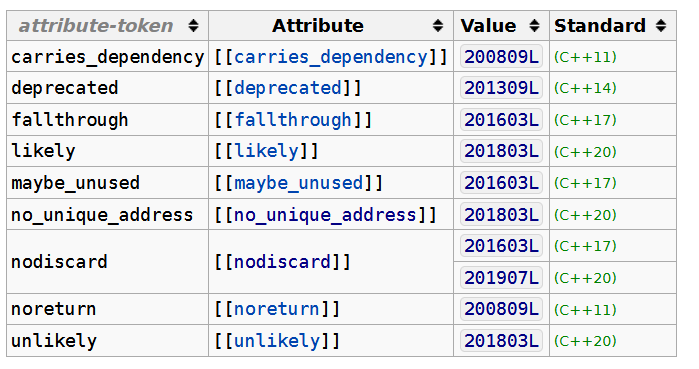
\includegraphics[width=0.8\textwidth]{content/5/chapter9/images/2.png}\\
属性的宏
\end{center}

下面是<version>标头及其宏的演示。我在全新的GCC、Clang和MSVC编译器上执行了这个程序,为GCC和Clang编译器使用了编译器资源管理器。/Zc:\_\_cplusplus标志允许\_\_cplusplus宏报告最新的C++语言标准支持。此外,我在所有三个平台上启用了C++20支持。这里,我只展示了对C++20核心语言的支持。

\hspace*{\fill} \\ %插入空行
\noindent
\textbf{GCC 10.2}

\begin{center}
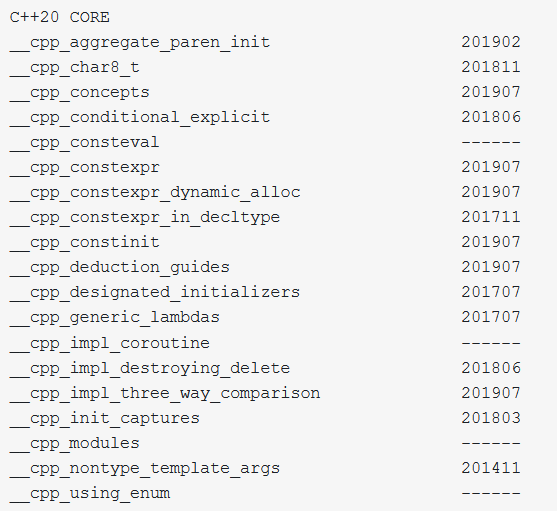
\includegraphics[width=0.6\textwidth]{content/5/chapter9/images/3.png}\\
\end{center}

\hspace*{\fill} \\ %插入空行
\noindent
\textbf{Clang 11.0}

\begin{center}
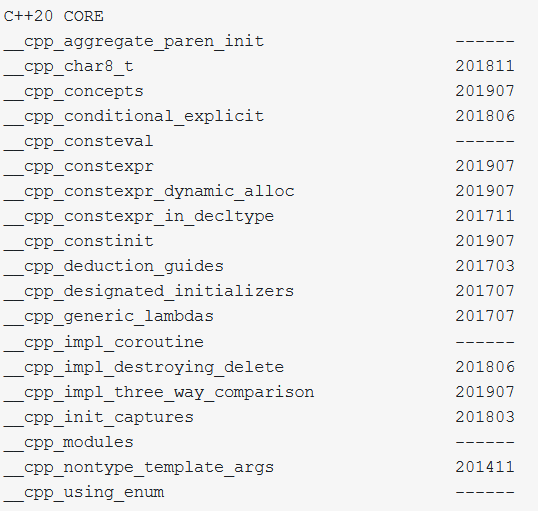
\includegraphics[width=0.6\textwidth]{content/5/chapter9/images/4.png}\\
\end{center}


\hspace*{\fill} \\ %插入空行
\noindent
\textbf{MSVC 19.27}

\begin{center}
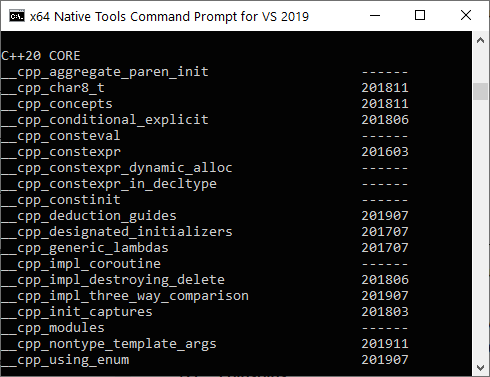
\includegraphics[width=0.6\textwidth]{content/5/chapter9/images/5.png}\\
\end{center}

这三张截图清楚地传达了这三巨头的信息:他们的C++20的核心语言支持,在2020年底时还是相当不错的。


